\chapter{Introduction}
\section{Background}
\label{background}
Electricity distribution networks, and the way in which they are managed, are currently going through a significant transition, with perhaps more change over the last ten years than in the previous hundred. %the sort of statement where a ref would help strengthen it, but OK not to have
Until recently, generation and load were largely viewed and managed separately: power was produced almost exclusively by large, centralised generating units, and was consumed by customers after routing via %traversing is not quite right word. reticulation... hmm???
the transmission and distribution networks. 
Networks were designed and built for demand profiles which were relatively stable over time, with demand forecasting at distribution feeder level required primarily for long term network planning purposes only. 
Increasingly, power is both consumed by customers connected to the distribution network and is also generated and manipulated by distributed energy resources (DER) within the distribution network, often behind the meter of individual consumers. 
The impact of increasing levels of DER in the system creates, among other things, both a need and an opportunity to more actively manage distribution networks, while also resulting in a generally less predictable net demand profile.

DERs are controllable devices in the power network that generate, store, and/or consume power. 
This includes solar photovoltaic generation (PV), battery storage, and electrical vehicles. 
In Australia, the dominant DER technology deployed to date is solar PV, with over 1.8 million systems now reportedly installed on residential properties \cite{apvi2017}. 
It is widely anticipated that battery storage and electrical vehicle uptake may be just as rapid \cite{bloomberg2018}.

The Tasmanian distribution network, meanwhile, is forecast to experience significant increases in these technologies by 2025: \\
\begin{itemize}
	\item 680\% increase in battery storage capacity (from 11MWh to 75MWh) \cite{Jacobs2017}
	\item 170\% increase in PV installation capacity (from 130MW to 220MW) \cite{Jacobs2017}
	\item 39\% of new car sales will be electrical vehicles - the highest in the country \cite{AEMO2016}
\end{itemize}

The changing nature of the distribution network presents an opportunity to maximize the use of existing assets by delaying the need for network augmentations, while also providing customers with a more reliable supply of power.
For example, batteries could be used to peak-shift, reducing maximum feeder load.
However, to achieve this reliably and with optimal use of available DER generally requires sophisticated methods to optimize the power flow to and from the distributed resources.

\begin{figure}[htbp]
	\centerline{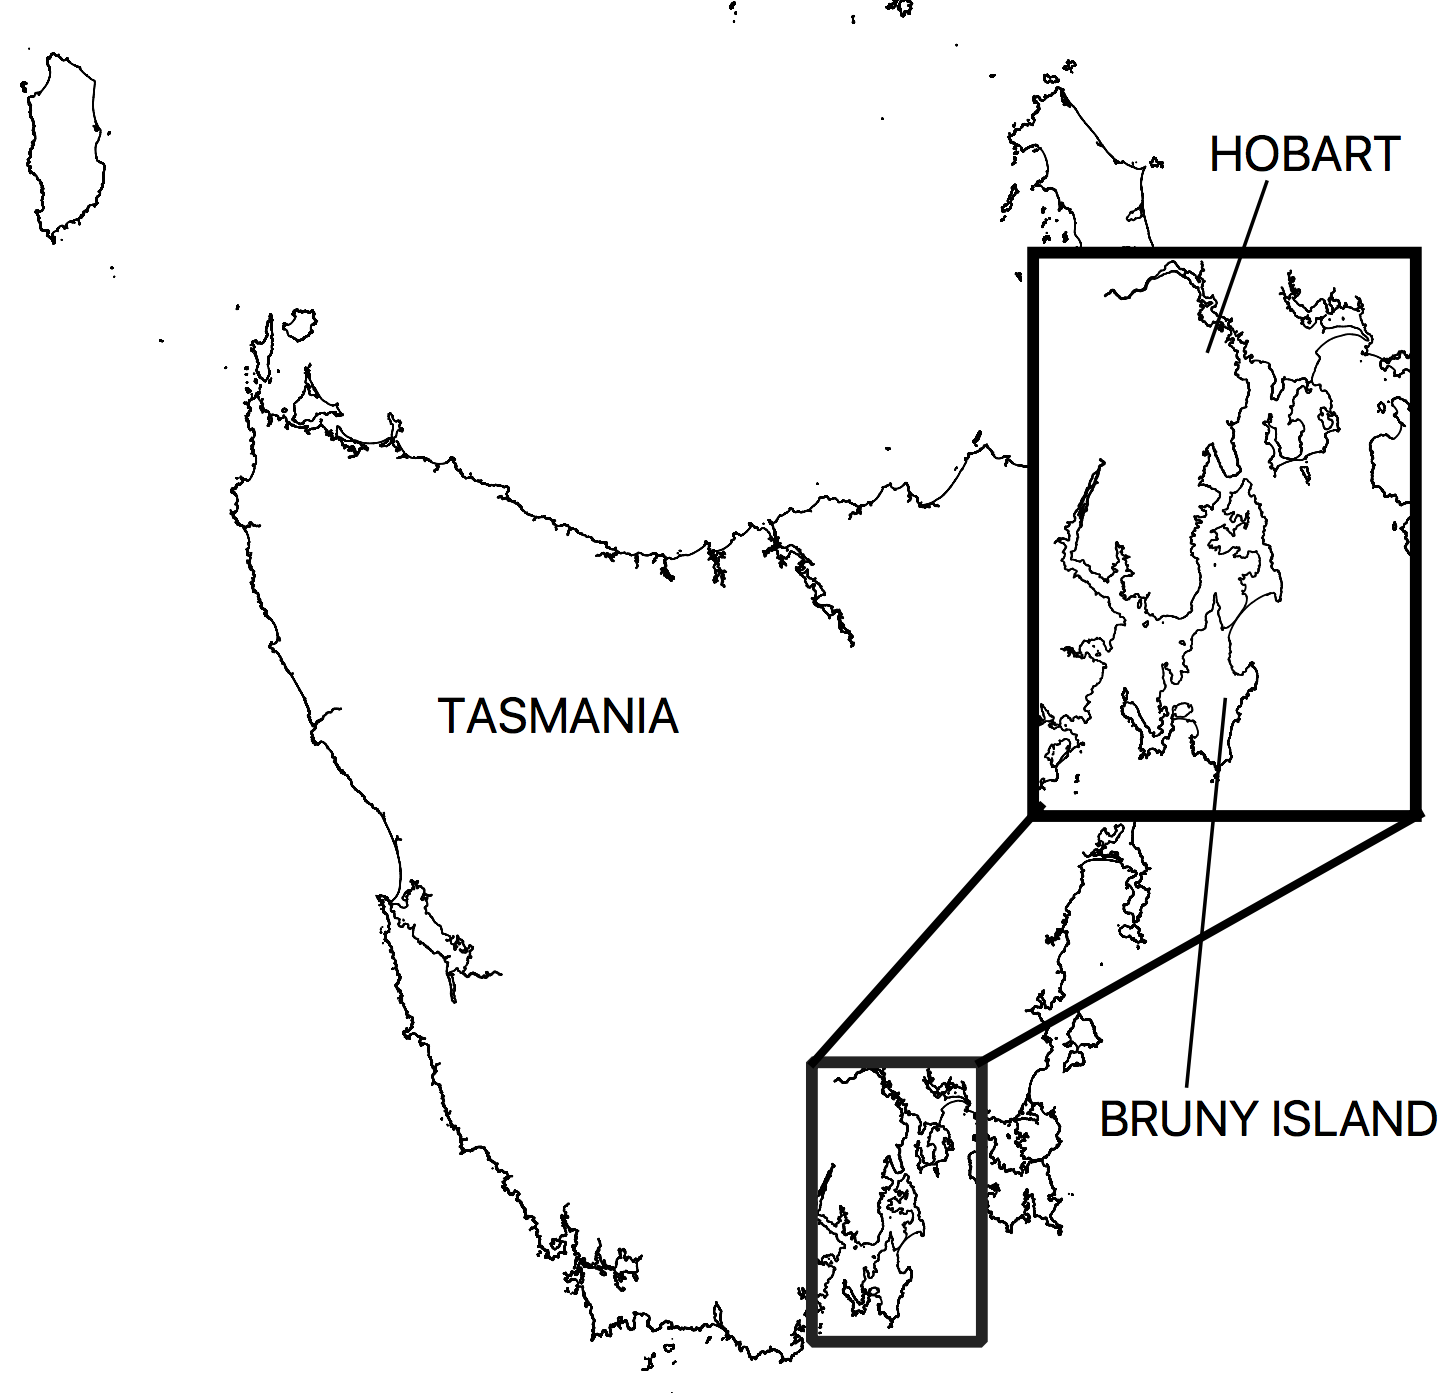
\includegraphics[width=.35\textwidth]{images/bruny_island_map.png}}
	\caption{Bruny Island in southeast Tasmania experiences significant increases in load during holiday periods and was used as a case study for the load forecaster.}
	\label{fig:bruny_map}
\end{figure}

One method to achieve this coordination of DER in distribution networks is presented in \cite{Scott2014} and has been implemented on Bruny Island, Tasmania as part of the CONSORT project (CONSumer energy systems providing cost-effective grid suppORT).
Bruny Island, shown in Figure \ref{fig:bruny_map}, is a popular holiday destination and during peak periods --- such as Easter morning and afternoon peaks --- the submarine feeder supplying the island becomes overloaded and is supplemented by a diesel generator located on the island.
The aim of the CONSORT project was to effectively peak shift the load away from the morning and afternoon peaks to prevent the use of the generator.

To fulfil such an objective while using the available distributed resources optimally, the CONSORT project relies upon having an accurate, online, 24-hour horizon forecast at the feeder level.
However, load forecasting methods commonly employed in industry are neither intended to forecast with high accuracy over a time period this short nor at the feeder level. \cite{CIGRE2016}.
An improved method for producing accurate feeder-level forecasts is not only highly desirable for this project, but will also in the future become a critical element of active distribution network management more generally.

In this thesis, a novel neural network-based day-ahead feeder level load forecasting system is developed, with its performance evaluated using ten years of historical demand data for training and testing. The forecaster is implemented live on Tasmania's Bruny Island distribution network, enabling the CONSORT project's residential battery systems to effectively support the network during periods of peak demand.

\section{State of the art in load forecasting}
What is clear throughout the literature is that there are a handful, perhaps a dozen or so, of clearly distinct techniques that are commonly applied to load forecasting.
However, these methods are nearly always mixed, matched, and combined to form a complete forecasting system.
As a result, there are a combinatorial number of approaches to forming a load forecasting system.
This section will attempt to cover only the most prolific techniques, and the examples cited will generally also employ techniques which have not been discussed. 
% The reader should not allow this to distract them from focussing on the technique being discussed.

\subsection{Load forecasting - definition and general remarks}
Before diving into state of the art load forecasting methods, it is important to first establish precisely what load forecasting is.
Load forecasting is the process of predicting the electricity demand in a particular area at each period over a planning horizon \citep{Weron2006}.
For example, a load forecast with a period of one hour and a horizon of 24 hours would forecast the load at each hour over the next 24 hours.
It is a specific case of time series forecasting.
Load forecasting can be broadly categorised into short-term (STLF), medium-term (MTLF), and long-term load forecasting (LTLF).
The exact horizon for each category differs between publications, but it is widely accepted that anything with a forecast horizon of less than 24 hours is short-term load forecasting.
This thesis will deal exclusively with STLF.
Generally a load forecast uses exogenous information as input, such as weather and date information, in order to produce a forecast.

The literature presents no single load forecasting system that is superior under all conditions.
A system that is well suited to forecasting load with a majority industrial customers may be poorly suited to forecasting load with a majority residential customers.
Perhaps it is more accurate to say that there is no single load forecasting problem - every feeder or network exhibits different patterns as a result of the different customers attached to it and thus must be treated as a separate problem.


\subsection{Load forecasting in industry}
In section \ref{background} it was stated that load forecasting methods commonly employed in industry neither intended to forecast with high accuracy over a 24 hour period nor at feeder level in the distribution network.
This is supported by a survey conducted by CIGRE in 2016 \citep{CIGRE2016} showing that, of 29 utilities, 79\% use load forecasting for long term planning and 32\% for short term operational planning.
Interestingly, this survey also found that the majority of load forecasting software is developed in-house, and the methodology used is usually revised at least every four years.


\subsection{Patterns in load profiles}
\label{patterns-profiles}
In a residential setting, such as a residential feeder, power is consumed as a result of customer actions - taking a shower causes the hot water system to consume power to reheat water, turning on a kettle or toaster causes power to be consumed, use of air conditioning results in power consumption, etc.
It is intuitive to expect that there would be patterns underlying these actions or behaviours; customers probably take showers more often in the morning, and when it is cold customers are probably more likely to turn on their heaters.
If the feeder in question happens to be in a popular holiday destination, then it might also be the case that overall more power is consumed during holiday periods as a result of more customers being in the area.
Any load forecasting system must be able to intrinsically model these underlying patterns if it is to effectively predict load.
\par
Before looking at load forecasting techniques and systems, we will first delve into the typically available data and investigate what patterns exist.
It needs to be kept in mind though that all conclusions presented here are general; they will likely vary between countries, cultures, and feeders.
Analysis of a specific feeder is undertaken in section \ref{bruny-data-analysis}.

\subsubsection{Calendar day}
The most significant factor contributing to a load profile is the calendar day \citep{Weron2006}.
Generally weekdays and weekends have differing load profiles, and even days during the week can be observed to have significantly different profiles.
It can be seen that seasonality normally plays a large role in load variation over a full year, but the extent depends on the location of the feeder.
Different feeders will experience changes in load due to warm and cool weather differently depending on customer behaviour.
Finally, holiday periods cause large deviations from standard profiles and can be difficult to predict due to the relatively few examples available.
Holidays sometimes also affect days adjacent to them, as people may also take these days off work.

\subsubsection{Weather}
Second to calendar day, the most significant factor behind the load profile is the weather \citep{Hippert2001}.
Typically temperature and humidity are considered the most influential, as they drive customers to use heating and cooling which both consume large amounts of power.
More recently, cloud cover and solar irradiance have become increasingly important as they affect rooftop photovoltaic (PV) generation \citet{AEMO2017}.
In regards to PV, it may be further necessary to model its uptake - solar capacity is increasing in Australia \citep{Jacobs2017} and so training data may need to be manipulated to reflect this.

\subsection{Similar day and clustering}
As discussed in section \ref{patterns-profiles}, a load profile is dependent primarily on the calendar day and the weather.
This fact can be used to form a rudimentary load forecasting system by simply finding a load profile from the past that has the most similar calendar day and weather properties to the period being forecast. 
Similarly, a clustering approach can be taken if it is assumed that load profiles will repeat themselves as a result of repeating weather and calendar day patterns.
\par
\citet{Rahman1993} used an expert-system based method to select a set of similar days from the past. 
These days were then modified by use of a lookup table based on differences in temperature and other exogenous factors between the similar and forecast period.
Finally, all similar days were regressed to form a forecast.
\par
\citet{Senjyu1998} used a weighted sum-squared-error between the maximum temperature, minimum temperature, and day type of the period being forecast and previous days to select the most similar five days from the past.
A fuzzy logic system was then used to generate weights to augment the similar days based on differences in weather and differences in load profile between the similar day and the day prior to the forecast day.
This was found to out-perform a more rudimentary systems which only used average load of the similar days.
The load being forecast was approximately 600MW.
\par
\todo[inline]{add some more. Next day load curve forecasting using recurrent neural network structure}


\subsection{Autoregressive integrated moving average}
Autoregressive integrated moving average (ARIMA) models, introduced by \citet{Box1970}, are used widely for time series forecasting \citep{Weron2006}. 
Generally, ARIMA models are used at the core of the forecasting system, and other methods are used in a supporting role. 
\par
\citet{Bennett2014} used an ARIMAX model to forecast the properties of the next day's load (next day peak demand, next day morning peak, and next day total energy usage). These properties were then provided to a neural network which selected the appropriate cluster for the day, whose load profile mean was then modified to better match the predicted properties.
\\
\citet{Karthika2017} used an ARIMA model to perform a preliminary load forecast, which was then augmented by a support vector machine to account for non-linear exogenous variables such as temperature and day of week.
\par
ARIMA-based models are complex and require a great deal of experience to effectively select appropriate parameters \citep{Desouky2000}.
\hl{todo expand on this lonely sentence}

\subsection{Support vector regression}
\todo[inline]{todo make consistent with Nomenclature chapter}
\todo[inline]{rewrite with notation and rationale from \cite{Goodfellow-et-al-2016} - their explanation is concise and eloquent}
Support vector regression (SVR) was introduced by \citet{Drucker1996} and has been applied widely to short-term load forecasting.
\par
\citet{Chen2004} applied a SVR model to predict the maximum daily load over a 31 day period, taking first place at the EUNITE Competition 2001.
\par
\citet{Ceperic2013} applied an ensemble of 24 SVR models to predict each hour of a 24-hour forecast.
This was found to out-perform \citet{RochaReis2005}, \citet{AMJADY2009}, and \citet{Deihimi2012} \hl{(todo expand on what these three papers actually are)}.
\par
In essence, SVR maps an input feature vector into a higher dimensional space and then applies linear regression.
\par
Consider a time series $X$ of input feature vectors with elements $X_{t}, X_{t-1}, ..., X_{0}$ and corresponding target $Y$ with scalar features $Y_{t}, Y_{t-1}, ..., Y_{0}$. SVR solves the following optimization problem
\begin{align}
& \min\limits_{\omega,b,\zeta,\zeta^{*}} & \frac{1}{2}\omega^T\omega + C\sum_{i=0}^{t}(\zeta_i+\zeta_i^*) \\
& \text{constrained by} & Y_i - (\omega^T\phi(X_i) + b) \leq \epsilon + \zeta_i^*,	\nonumber \\
                       && (\omega^T\phi(X_i)+b)-Y_i\leq\epsilon+\zeta_i,	\nonumber \\
                       && \zeta_i \geq 0, \zeta_i^* \geq 0 \nonumber
\end{align}
where $\phi(X_i)$ is the mapping of the input feature to a higher dimensional space, $\epsilon$ is the diameter of the $\epsilon$-insensitive tube $|y - (\omega^T\phi(X) + b)| \leq \epsilon$, $\zeta_i$ and $\zeta_i^*$ are slack variables, $C$ is the error penalization cost hyper-parameter, $b$ is the bias parameter, and $\omega$ is the weight parameter.
\par
Intuitively, this optimization problem solves for $\omega$ and  $b$ such that the distance of training samples outside of the $\epsilon$-insensitive tube is minimized. The distance above and below the tube is given by the slack variables $\zeta_i$ and $\zeta_i^*$. Samples which are within the tube do not contribute to the minimization problem. The $\frac{1}{2}\omega^T\omega$ is a regularization term that penalizes the model for producing large magnitude weights, which are associated with over-fitting \citep{Drucker1996}.
\par
Solving the Lagrangian dual of the above optimization problem leads to the following
\begin{equation}
Y_n = \sum_{i=0}^{t}(\alpha_i - \alpha_i^*)K(X_i, X_n) + b
\end{equation}
where $\alpha_i$ and $\alpha_i^*$ are Lagrange multipliers, and $K(X_i, X_n) = \phi(X_i)^T\phi(X_n)$ is a kernel function. Using a kernel function avoids computing $\phi(X_n)$, which may be intractably large, and instead computes the transformation in a lower dimensional space.

\subsection{Gradient boosting}

\subsection{Artificial Neural Network}
\todo[inline]{clarify feedforward/recurrence and unrolling of RNN when defining ANN}
An artificial neural network (ANN) is a method for computation based loosely on biological brains \citep{negnevitsky2005artificial}.
An ANN is simply a function approximator; given a function $f^*(\vx)$, an ANN defines an approximation function $f(\vx; \vtheta)$ where $\vtheta$ is a (usually learned) set of parameters that lead to the best approximation of $f^*$ \citep{Goodfellow-et-al-2016}. 
\par
ANNs have achieved state of the art performance in handwriting recognition \citep{2017arXiv171009829S}, machine translation \citep{Vaswani2017}, speech recognition \citep{Chiu2017}, and speech synthesis \citep{DBLP:journals/corr/OordDZSVGKSK16}.
ANNs have been demonstrated to out-perform ARIMA models for electricity time series price forecasting \citep{Mandal2010}.
For short-term time series vehicle traffic forecasting, ANNs have been shown to outperform both ARIMA and SVM (SVR) models \cite{Zhao2017}.
\par
\citet{Chen2010} employed a wavelet neural network and similar day selection to perform a load forecast with a 24-hour horizon and 1-hour resolution.
The load being forecast was on the order of $10^4$ MW and the forecast was performed only once per day, at 9am.
The authors calculated the wind chill temperature, based on ambient temperature and wind speed, and transformed it to have a linear relationship with load before using it as an input to the system.
\par
\citet{Kong2017} and \citet{Kong2018} applied a long short term memory recurrent neural network for short term load forecasting of individual household load and found that it out-performed simpler multilayer perceptron models and clustering-only methods.
\par
\hl{ add also} \citep{Mansouri2014}.
\par
Generally, ANNs are formed by combining many fundamental sub-functions in a graph-like manner. 
An example is the multilayer perceptron.
Consider a single perceptron, shown in figure \ref{fig:single-perceptron}.
This single perceptron simply takes the weighted sum of all inputs and applies an activation function, usually differentiable and highly non-linear, to produce an output $a$.
A multilayer perceptron is formed by structuring individual perceptrons in layers and cascading them so that the outputs of the perceptrons in one layer are the inputs to the perceptrons in the next layer, as shown in figure \ref{fig:mlayer-perceptron} where the squares and circles are individual perceptrons and the lines indicate connections from the output of one perception to the input of the next.
The weights W are mapped to elements in the parameter vector $\vtheta$.
The hidden layer can be repeated any number of times, allowing the neural network to be written in the form $f(\vx) = f^n(f^{\ldots}(f^1(\vx)))$.
The exception to this is recurrent neural networks, where the outputs of sub-functions in the network form cycles.
\todo[inline]{todo reproduce figure \ref{fig:simple-ann} myself.}
\begin{figure}[htbp]
	\centering
	\subfigure[from \citet{Zainal-Mokhtar2013}.]{
		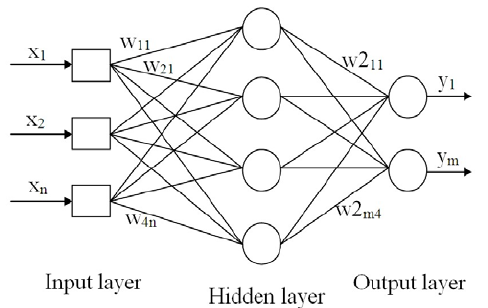
\includegraphics[width=.35\textwidth]{images/A-schematic-diagram-of-a-Multi-Layer-Perceptron-MLP-neural-network.png}
		\label{fig:mlayer-perceptron}}
	%\vfil
	\quad\quad
	\subfigure[from \citet{Deshpande2017}.]{
		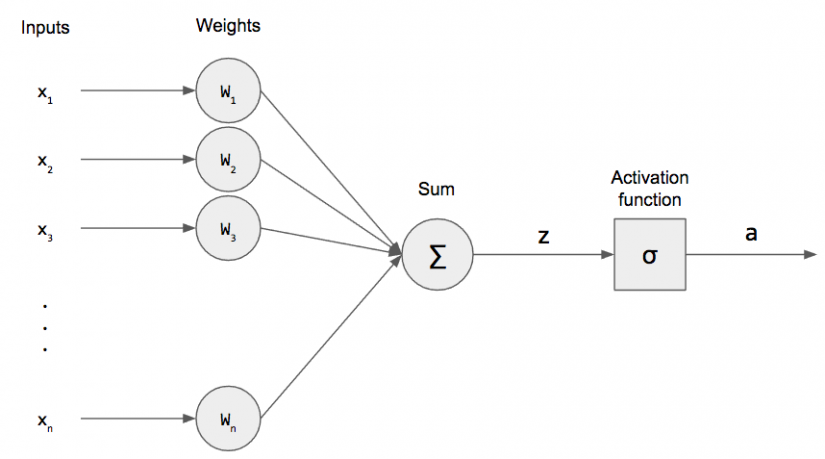
\includegraphics[width=.35\textwidth]{images/Single-Perceptron-825x459.png}
		\label{fig:single-perceptron}}
	\caption{(a) A multilayer perceptron comprised of layers of individual perceptrons. (b) An individual perceptron. TODO: reproduce myself}
	\label{fig:simple-ann}
\end{figure}
% directed acyclic graph, where nodes in the graph represent operations on data, and edges represent the flow of data through the graph. 
%This thesis will restrict itself to discussion of feedforward neural networks. 
%A feedforward neural network is an ANN where 
%Any recurrence will be unrolled to form a feedforward network. A feedforward 

\par
The set of parameters $\vtheta$ is usually learned, or trained, by stochastic gradient descent \citep{Bottou2011}.
Consider an ANN producing an approximated output $\hat{\vy} = f(\vx; \vtheta)$ and a cost function $J(\vy, \hat{\vy}) = J(\vy, \vx, \vtheta)$, with  $J$ being a differentiable function of its inputs, $\vy$ being the correct output of $f^*$, and $\vtheta$ being randomly initialized.
The cost function produces a scalar describing the error between $\vy$ and $\hat{\vy}$.
A common example of this is sum squared error, where $J(\vy, \hat{\vy}) = \sum_{n=o}^{i}(|\vy_n - \hat{\vy}_n|^2)$.
The gradient of $J$ with respect to the parameters is given by $\nabla_{\vtheta}J(\vy, \vx, \vtheta)$ and indicates the direction in which to move $\vtheta$ in order to increase $J$.
By iteratively applying $\vtheta = \vtheta - \epsilon \nabla_{\vtheta}J(\vy, \vx, \vtheta)$ (where $\epsilon$ is a scalar constant referred to as the learning rate), the value of $\vtheta$ will be modified such that $J(\vy, \vx, \vtheta)$ is minimized - thus maximizing the approximation accuracy of $f$.
$\vx$ and $\vy$ must be a randomly selected pair from the training set in order for this training process to represent the whole training dataset.
Whether this minimization lands on a global or local minimum is dependant on the function $J$.
\par


\section{Problem formation and scope}
\label{scope}
The aim of this thesis is to build upon existing research and develop a load forecasting system which can predict future load based on weather, holiday periods, car movement, and other factors. 
Bruny Island and the NAC will be used as a case study. 
The forecasting system is expected to be equally applicable to any power system network.
\\
Specifically, the system will have the following properties:
\begin{itemize}
	\item The system will produce a forecast up to 24 hours in the future in 15- to 60-minute intervals. This will be a rolling forecast that can be re-calculated at any time.
	\item The forecast will be able to begin from any point time.
	\item The forecast will predict load in kVA at each interval.
	\item The forecast system will be aimed at predicting aggregate load at the feeder level. That is, between approximately 0.5 and 10MVA.
	\item The forecast system will be especially tuned to predict load during holiday periods.
\end{itemize}
